\documentclass[../sparc.tex]{subfiles}
\graphicspath{{\subfix{../images/}}}
\begin{document}

%%%%%%%%%%%%%%%%%%%%%%%%%%%%%%%%%%%%%%%%%%%%%%%%%%%%%%%%%%%%%%%%%%%%%%%%%%%%%%%%
\section{Analog-to-digital converter}

As we could see in the section \ref{section:analog-ports}, values read from an
analog port lie in range that spans from 0 to 1023.  The number 1023 is
suspiciously close to the number 1024, which can be found very often in
programming -- it's no wonder as it is a power of 2 ($2^{10}$.)

If we track this trace down the road, we would see that an analog port somehow
converts the input analog signal to the digital (binary) representation that we
see in the program.

If we allocate 10 bits for storing the data, we can encode up to $2^{10} = 1024$
combinations of zeroes and ones -- thus the maximal value 1023 as we must
consider that we start from zero, which is the one of the possible values.

The analog-to-digital conversion is performed by the component that is called
\emph{analog-to-digital converter} (usually shortened to ``ADC''.)  The ADC role
can be played by either a separate microchip or by the micro-controller itself.
The ADC can be depicted schematically as is shown on the
fig. \ref{fig:adc-schematics}.

\begin{figure}[ht]
  \centering
  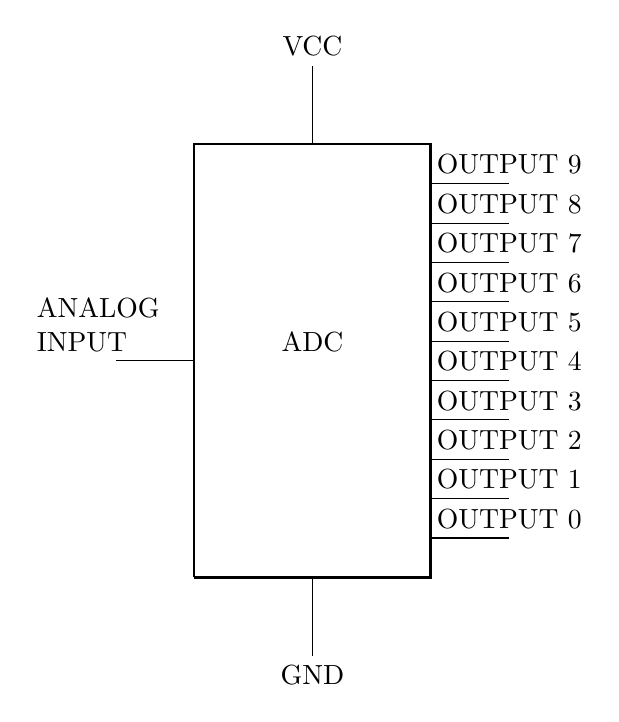
\begin{tikzpicture}
    \draw[thick] (0, 0) -- (0, 5.5) -- (3, 5.5) -- (3, 0) -- (0, 0);
    \draw (1.5, 2.75) node[right, above] {ADC};
    \foreach \n/\y in {0/0.5, 1/1, 2/1.5, 3/2, 4/2.5, 5/3, 6/3.5, 7/4, 8/4.5, 9/5} {
      \draw (3, \y) -- (4, \y) node[right, above] {OUTPUT \n};
    };
    \draw (0, 2.75) -- (-1, 2.75) node[left, above, text width=2cm] {ANALOG INPUT};
    \draw (1.5, 5.5) -- (1.5, 6.5) node[right, above] {VCC};
    \draw (1.5, 0) -- (1.5, -1) node[right, below] {GND};
  \end{tikzpicture}
  \caption{Schematic depiction of the analog-to-digital converted (ADC.)}
  \label{fig:adc-schematics}
\end{figure}

The ADC takes some analog signal into the input (``ANALOG INPUT'') and encodes
it in each moment in time as the sequence of logical levels: ``HIGH'' (``1'')
and ``LOW'' (``0''.)  The ADC itself requires the power supply which is provided
through ``VCC'' and ``GND'' pins.

\example{ Let's suppose we supplied 2.5V to the ADC input.  The ADC outputs the
  binary value ``1000000000'' which represents the number $2^9 = 512$ -- that can
  be read in the program running on a micro-controller. }

The conversion of an analog signal to a digital form inside an ADC is done in
three steps:

\begin{enumerate}

\item \textbf{Sampling.}  During this step ADC takes samples from the input
  analog signal at regular intervals of time (see \ref{fig:discretization}.)

  \begin{figure}[h]
    \centering
    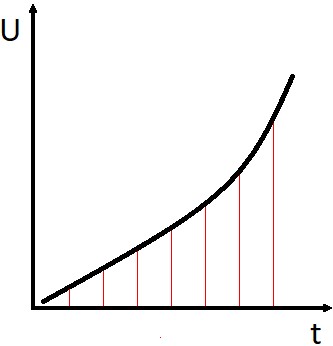
\includegraphics[width=8cm]{discretization}
    \caption{Sampling.}
    \label{fig:discretization}
  \end{figure}

  The frequency of those intervals is called \emph{sampling rate}.

\item \textbf{Quantization.}  Acquired values are replaced with the closest
  values from the set of possible values -- \emph{quantization levels}.

  \begin{figure}[h]
    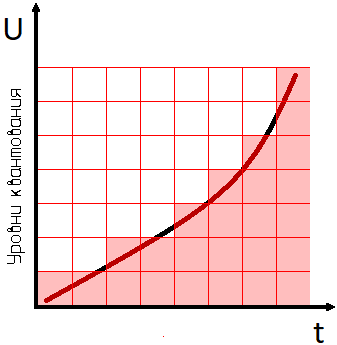
\includegraphics[width=8cm]{quantization}
    \caption{Quantization.}
    \label{fig:quantization}
    \centering
  \end{figure}

\item \textbf{Encoding.}  Binary codes are assigned to the resulting values (see
  \ref{fig:coding}.)

  \begin{figure}[h]
    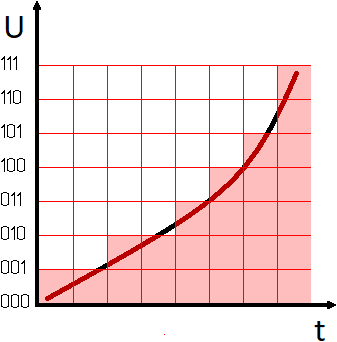
\includegraphics[width=8cm]{coding}
    \caption{Encoding.}
    \label{fig:coding}
    \centering
  \end{figure}

  The higher the sampling rate and the more quantization levels are available,
  the more precise the analog-to-digital conversion.

\end{enumerate}

\end{document}

